%%%%%%%%%%%%%%%%%%%%%%%%%%%%%%%%%%%%%%%%%%%%%%%%%%
%% Layer Overview
%%%%%%%%%%%%%%%%%%%%%%%%%%%%%%%%%%%%%%%%%%%%%%%%%%
% In this section, the layer is described in terms of the hardware and software design. Specific implementation details, such as hardware components, programming languages, software dependencies, operating systems, etc. should be discussed. Any unnecessary items can be ommitted (for example, a pure software module without any specific hardware should not include a hardware subsection). The organization, titles, and content of the sections below can be modified as necessary for the project.
The Movement Subsystem controls the rover's motion by managing speed, direction, and collision avoidance. It receives navigation commands from the Raspberry Pi and sends signals for motor control, ensuring responsive navigation.

%%%%%%%%%%%%%%%%%%%%%%%%%%%%%%%%%%%%%%%%%%%%%%%%%%
%% Layer Description
%%%%%%%%%%%%%%%%%%%%%%%%%%%%%%%%%%%%%%%%%%%%%%%%%%

% \subsection{Layer Hardware}
% A description of any involved hardware components for the layer. For example, if each subsystem is a software process running on an embedded computer, discuss the specifics of that device here. Do not list a hardware component that only exists at the subsystem level (include it in the following sections).

% \subsection{Layer Operating System}
% A description of any operating systems required by the layer.

% \subsection{Layer Software Dependencies}
% A description of any software dependencies (libraries, frameworks, etc) required by the layer.

%%%%%%%%%%%%%%%%%%%%%%%%%%%%%%%%%%%%%%%%%%%%%%%%%%
%% Subsystem X - Template
%%%%%%%%%%%%%%%%%%%%%%%%%%%%%%%%%%%%%%%%%%%%%%%%%%

% \subsection{Subsystem X}
% Descibe at a high level the purpose and basic design of this subsystem. Is it a piece of hardware, a class, a web service, or something else? Note that each of the subsystem items below are meant to be specific to that subystem and not a repeat of anything discussed above for the overall layer.

% \begin{figure}[h!]
% 	\centering
%  	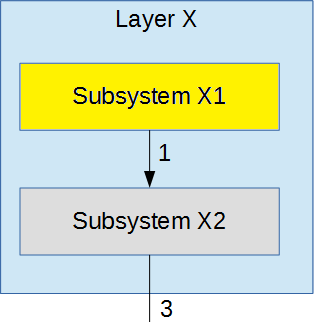
\includegraphics[width=0.60\textwidth]{images/subsystem}
%  \caption{Example subsystem description diagram}
% \end{figure}

% \subsubsection{Subsystem Hardware}
% A description of any involved hardware components for the subsystem.

% \subsubsection{Subsystem Operating System}
% A description of any operating systems required by the subsystem.

% \subsubsection{Subsystem Software Dependencies}
% A description of any software dependencies (libraries, frameworks, design software for mechanical parts or circuits, etc) required by the subsystem.

% \subsubsection{Subsystem Programming Languages}
% A description of any programming languages used by the subsystem.

% \subsubsection{Subsystem Data Structures}
% A description of any classes or other data structures that are worth discussing for the subsystem. For example, data being transmitted from a microcontroller to a PC via USB should be first be assembled into packets. What is the structure of the packets?

% \subsubsection{Subsystem Data Processing}
% A description of any algorithms or processing strategies that are worth discussing for the subsystem. If you are implementing a well-known algorithm, list it. If it is something unique to this project, discuss it in greater detail.



%%%%%%%%%%%%%%%%%%%%%%%%%%%%%%%%%%%%%%%%%%%%%%%%%%
%% Subsystem 1 - Microcontroller
%%%%%%%%%%%%%%%%%%%%%%%%%%%%%%%%%%%%%%%%%%%%%%%%%%

\subsection{Microcontroller}
The microcontroller \cite{TM4C} is a hardware component responsible for processing commands and controlling the rover's movement. It manages communication between the control systems and the motor drivers, sending directional and speed commands. Additionally, it handles sensor inputs for obstacle detection and emergency stops, ensuring safe and efficient operation.

\begin{figure}[h!]
	\centering
 	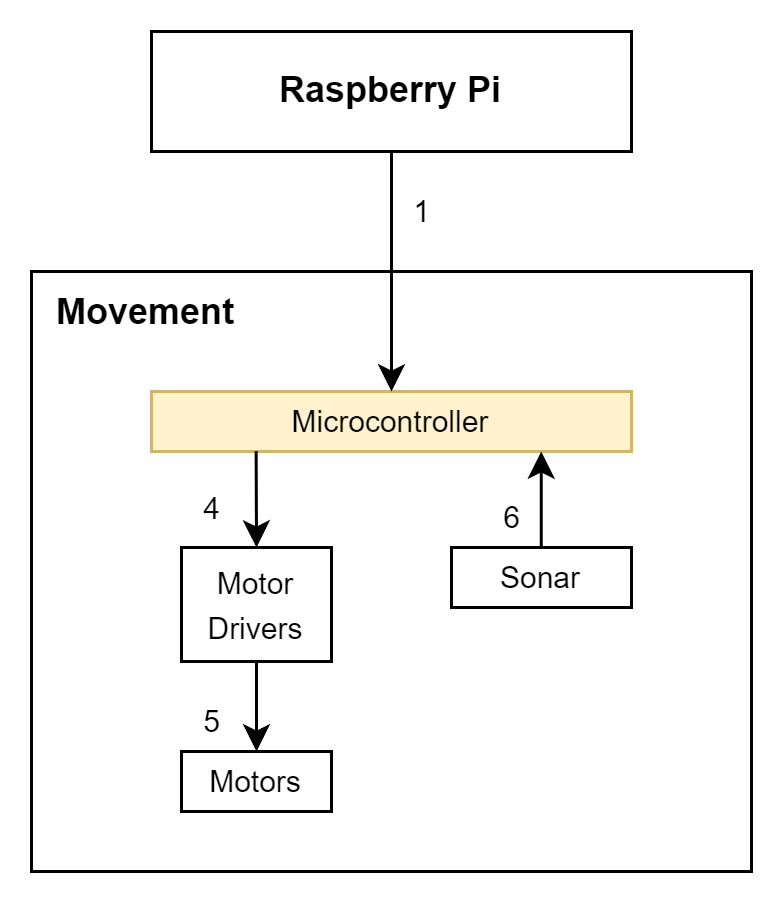
\includegraphics[width=0.60\textwidth]{images/movement/1_microcontroller.jpg}
 \caption{Movement Layer - Microcontroller Subsystem}
\end{figure}

\subsubsection{Subsystem Hardware}
\begin{itemize}
    \item TM4C RedBoard - A microcontroller with built-in UART and GPIO modules, responsible for processing motor control commands and handling sensor inputs (Figure \ref{fig:Movement Layer - Microcontroller Circuit}).
\end{itemize}

\subsubsection{Subsystem Software Dependencies}
TI Driver Library (Tivaware) - Provides low-level control over the TM4C RedBoard's peripherals, including UART and GPIO.

\subsubsection{Subsystem Programming Languages}
The TM4C RedBoard firmware uses C to implement the communication protocols and to control movement functions.

\subsubsection{Subsystem Data Structures}
\begin{itemize}
    \item (4x) 1-bit input GPIO control signals, one for each movement direction.
    \item 8-bit control packets are sent via UART to regulate each motor. Each packet consists of a single byte representing motor-specific commands such as speed and direction. Transmission occurs at 9600 baud with 5V, 8N1 settings, controlling one motor per packet.
\end{itemize}

\subsubsection{Subsystem Data Processing}
The microcontroller polls movement direction inputs every 100ms, capturing the required state and transmitting four motor control commands (one per motor).
\newpage



%%%%%%%%%%%%%%%%%%%%%%%%%%%%%%%%%%%%%%%%%%%%%%%%%%
%% Subsystem 2 - Motor Drivers
%%%%%%%%%%%%%%%%%%%%%%%%%%%%%%%%%%%%%%%%%%%%%%%%%%

\subsection{Motor Drivers}
The motor drivers \cite{Sabertooth} are hardware components that regulate power to the DC motors based on control packets received from the TM4C RedBoard. These are Sabertooth controllers that process incoming commands to adjust motor speed and direction. They ensure efficient and precise movement of the rover.

\begin{figure}[h!]
	\centering
 	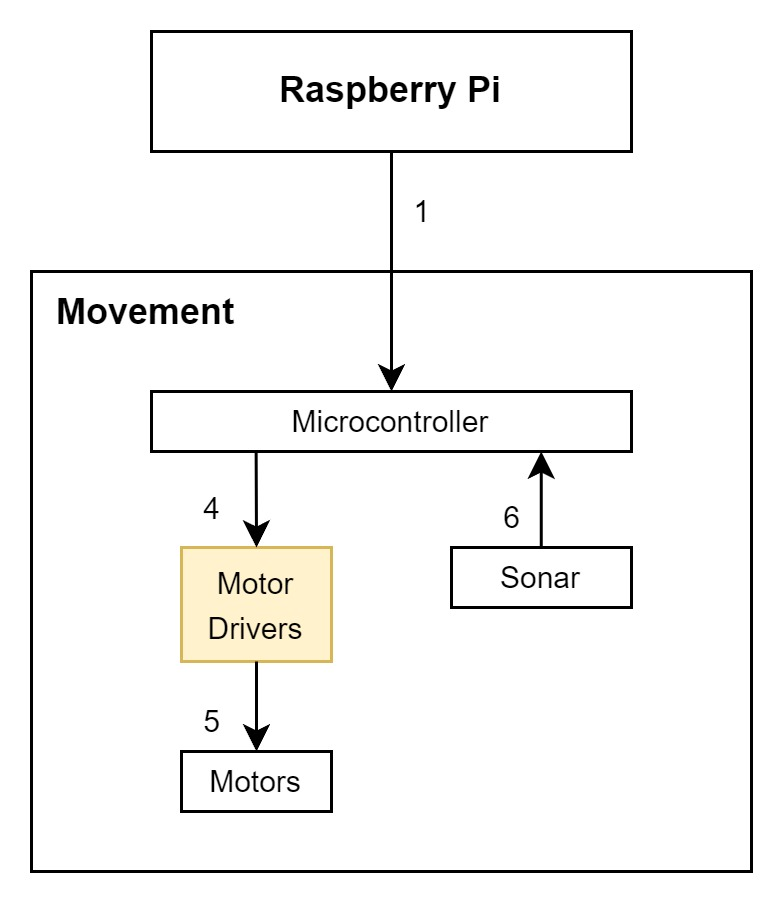
\includegraphics[width=0.60\textwidth]{images/movement/2_motordriver.jpg}
 \caption{Movement Layer - Motor Drivers Subsystem}
\end{figure}

\subsubsection{Subsystem Hardware}
\begin{itemize}
    \item Two Sabertooth 2x25 Motor Controllers - High-performance dual motor drivers that receive UART commands from the TM4C RedBoard. Each controller independently drives two motors, enabling precise movement control (Figure \ref{fig:Movement Layer - Motor Drivers Circuit}).
\end{itemize}

\subsubsection{Subsystem Data Structures}
\begin{itemize}
    \item 8-bit control packets regulate motor operations. Each packet consists of a single byte representing speed and direction commands. The packets are received over UART at 9600 baud with 3.3V, 8N1 (1 start bit, 8 data bits, 1 stop bit) settings, controlling one motor per packet.
\end{itemize}

\subsubsection{Subsystem Data Processing}
Each Sabertooth controller processes incoming UART packets every 100ms. Two packets (one per motor) are received per controller, spaced 50us apart to ensure proper sequencing and avoid command overlap.
\newpage



%%%%%%%%%%%%%%%%%%%%%%%%%%%%%%%%%%%%%%%%%%%%%%%%%%
%% Subsystem - Motors
%%%%%%%%%%%%%%%%%%%%%%%%%%%%%%%%%%%%%%%%%%%%%%%%%%

\subsection{Motors}
The motors are the primary actuators responsible for the physical movement of the rover. These are high-performance DC motors controlled by the motor drivers to achieve the desired speed and direction. The motors receive regulated power from the motor drivers, ensuring smooth movement.

\begin{figure}[h!]
\centering
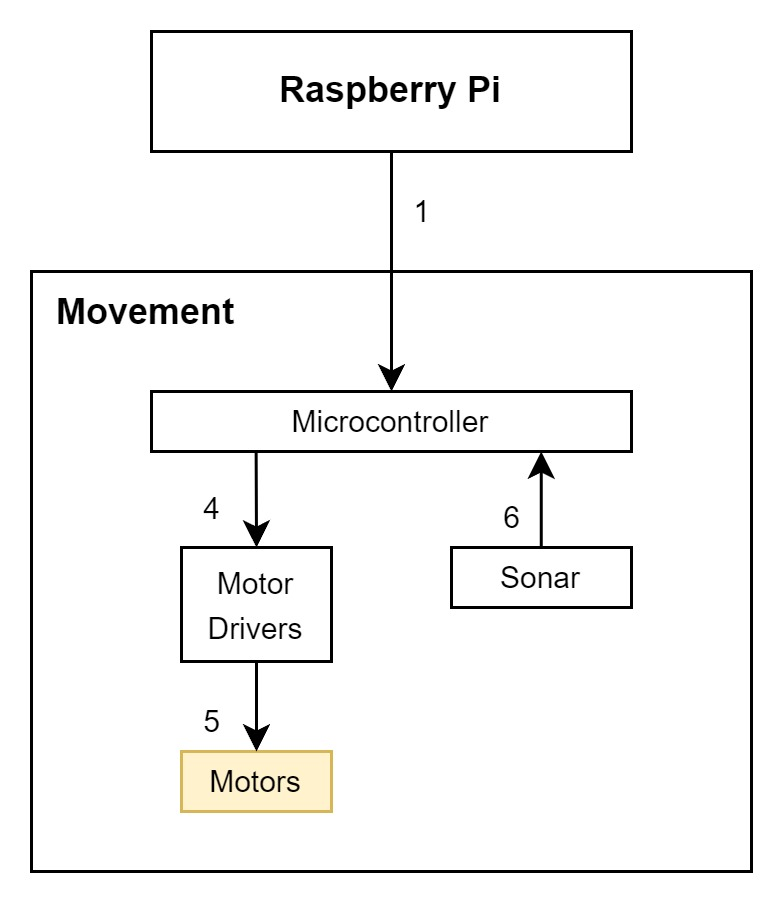
\includegraphics[width=0.60\textwidth]{images/movement/3_motors.jpg}
\caption{Movement Layer - Motors Subsystem}
\end{figure}

\subsubsection{Subsystem Hardware}
\begin{itemize}
\item Four DC Motors - Generate the mechanical power required for rover movement. The motors are grouped into front and rear pairs, each controlled independently by the motor drivers to regulate speed and direction.
\end{itemize}
\newpage



%%%%%%%%%%%%%%%%%%%%%%%%%%%%%%%%%%%%%%%%%%%%%%%%%%
%% Subsystem - Sonar (Last-Case Obstacle Detection)
%%%%%%%%%%%%%%%%%%%%%%%%%%%%%%%%%%%%%%%%%%%%%%%%%%\

\subsection{Sonar}
The Sonar subsystem utilizes ultrasonic sensors to detect obstacles in the rover's path. The system works by emitting sound waves and measuring the time it takes for the waves to bounce back after hitting an obstacle. The data is processed to determine the distance to the nearest object, enabling the rover to take last-minute actions to avoid collisions.

\begin{figure}[h!]
\centering
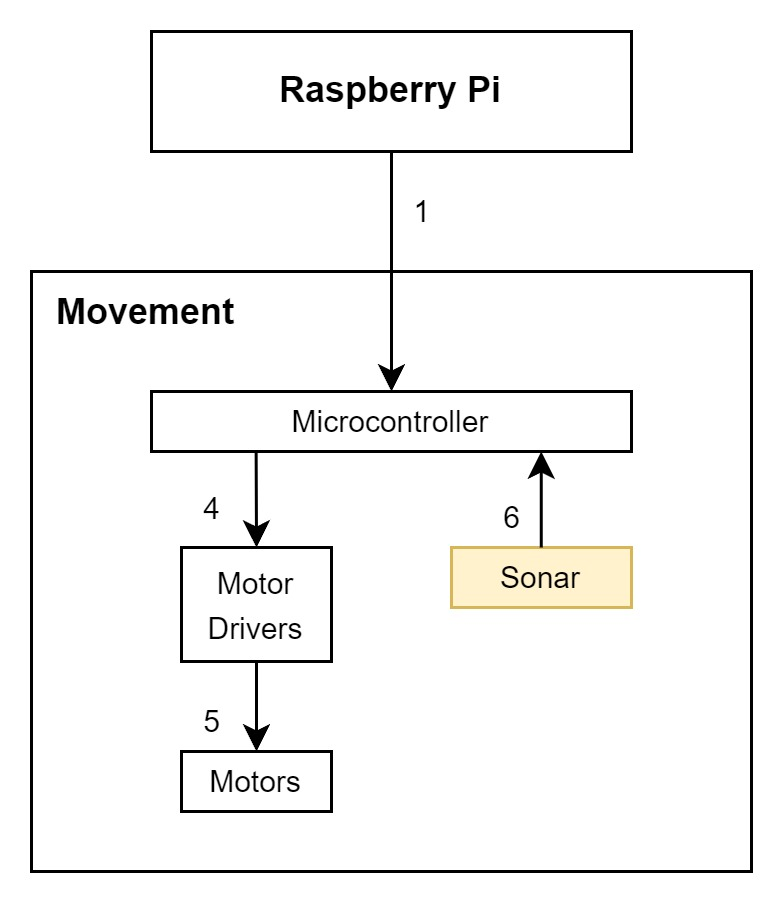
\includegraphics[width=0.60\textwidth]{images/movement/4_sonar.jpg}
\caption{Movement Layer - Sonar Subsystem}
\end{figure}

\subsubsection{Subsystem Hardware}
\begin{itemize}
    \item Ultrasonic Distance Sensor (HC-SR04) - Commonly used sensors that emit sound waves and listen for the echo, allowing for precise distance measurements to obstacles in the rover's path.
\end{itemize}

\subsubsection{Subsystem Data Structures}
\begin{itemize}
    \item 8-bit distance value (in centimeters) transmitted from the sensor to the microcontroller. This value represents the distance to the nearest obstacle detected by the sonar.
\end{itemize}

\subsubsection{Subsystem Data Processing}
The microcontroller sends a 10us pulse to the sensor's trigger pin, which causes the sensor to emit an ultrasonic wave. The time taken for the echo to return is measured to compute the distance. The system continuously polls the sensor at regular intervals (every 100ms) to update the obstacle detection distance. If an obstacle is detected within a defined threshold (50 cm), the rover will stop.
